\section{From Local Opportunity to Realized Gain}
\label{sec:diagnoses}
We test output qualification, frozen path prediction and sampled intervention effects, then examine realized cost on a qualified path. Figure~\ref{fig:translation} shows the original B570 discovery, freeze and reserved test; later studies use their own tasks and gates.

\subsection{Execution-path qualification}
\label{sec:admissibility}
Figure~\ref{fig:verification}A retains eleven historical target-forward proxy cells. Metal $\vTwo\approx1.02$--$1.08$, near-step RTX batching, and B570 fast 1.24--1.64 versus serialized \BvShort--\BvLong\ describe different runs and contexts. Lower proxy values mean cheaper target-forward work relative to one-token decode. These measurements omit integration, cannot replace complete $\rtarget$, and have no same-study matched cost/qualification tradeoff with Panel B.

Original RTX and B570 direct-ID campaigns each use 30 prompts $\times$ three, with no timing and a 90/90 gate. RTX matches \DIRTXBatchedPairs/90 batched and \DIRTXSerializedPairs/90 serialized; only serialization qualifies. B570 matches \DIBFastPairs/90 fast and \DIBSerializedPairs/90 serialized; both are blocked. Historical and fresh B570 60/90 counts are different comparisons. Repeat stability does not imply reference equality; Figure~\ref{fig:verification}A/B cannot form a matched speed/qualification tradeoff. RTX V4 below measures a new matched study, without certifying historical timing.

\subsection{B570 prediction and sampled live intervention}
\label{sec:b570mechanism}
A target-only harness first reproduces 90/90 UB128 reference sequences. H1 target-only UB1 matches 36/36 sequences on 12 exposed discovery tasks; its frozen tree selects H1, leaving H2 unrun. After conservative exposure exclusion, 24 reserved tasks are selected. H1 freezes before reserved inference and all 72 full predictions freeze before reserved live. Prediction/live agrees 72/72 over three stable runs per prompt, including four reference-divergent prompts (12 runs); the same-set UB128 reference agrees only 60/72 and remains \emph{BLOCKED}. All these reserved arrays reach 128 IDs. The predictor could have failed on any reserved sequence; its success establishes predictive path sufficiency on this B570 stack, not a unique numerical cause. The earlier serialized 78/90 gate has a different task set and reference comparison.

A separately frozen fork study uses 24 new prompts $\times$ three, sampling each first verification block after at least 64 committed IDs. UB1/UB128 branches share checked KV, prefix, positions, proposals and cloned sampler state. Scores change at \FUForkScores/72 forks, but raw top-one and actual immediate decisions change at \FUForkImmediate/72. Later complete trajectories differ in \FUForkLater/72 runs on \FUForkLaterPrompts/24 prompts. Repeats and within-block events are correlated.

The alternate branch restores draft state and continues with UB128 target blocks; later proposals follow its own live history. Delayed differences therefore cannot be attributed to the sampled block alone or treated as immediate reference restoration. Existing-record analysis of 216 correlated raw-logit rows gives median absolute top-one score change \DerScoreAbsMedian; top-one IDs remain unchanged. The six sensitive prompts first diverge 10--50 positions after the fork. Appendix P retains all score/margin summaries, positions and clone/R0 controls. These findings identify no unique operation or whole-generation null effect.

\subsection{RTX same-set trajectory discriminator}
\label{sec:rtxreplay}
Earlier RTX H1 target-only UB2 fails discovery at 24/36 and executes no reserved runs. Separate V2 H2/live, R\_ONLY/live and H2/R\_ONLY match 72/72, with UB1 reference/live 60/72. H2's draft-only P and target-only R processes compute their own feedback and decisions; fresh R\_ONLY reads the sealed proposal tape sequentially, while native live imports no tape. This is application/API orchestration independence on shared llama.cpp/GGML/CUDA routines. V2 lacked a same-set target-only competitor.

V4 fills that gap on all 19 remaining exposure-audited tasks. Four pre-live conditions---UB1 reference, target-only UB2, H2 and fresh R\_ONLY---produce 228 complete arrays; all predictions and tapes are frozen and remotely retrieved before 57 native batched live runs. Table~\ref{tab:rtxv4trajectory} contrasts the predefined candidates. UB2/live matches only 51/57 on 17/19 prompts; H2/live, R\_ONLY/live and H2/R\_ONLY each match 57/57. Reference/live is 51/57, including two reference-divergent prompts that both replay programs predict. All five conditions are repeat-stable.
\begin{table}[t]
\caption{RTX V4 prospective full-array prediction against native batched live. All rows use the same 19 prompts $\times$ three; predictions precede live. These are prediction comparisons, not reference qualification.}
\label{tab:rtxv4trajectory}
\centering
\begin{tabular}{@{}lrr@{}}
\toprule
Predictor / comparator & Pairs / 57 & Prompts / 19 \\
\midrule
Target-only UB2 & 51 & 17 \\
Independent P/R (H2) & 57 & 19 \\
Fresh R\_ONLY & 57 & 19 \\
UB1 reference & 51 & 17 \\
\bottomrule
\end{tabular}
\end{table}


Equal aggregate counts do not make UB2 and reference the same predictor: UB2 fails on /15 and /25, reference on /15 and /18. The test rejects this specified UB2 candidate's full-cohort sufficiency. It does not reject every target-only hypothesis or prove proposal/history necessary, minimal or unique. Replay uses drafting to construct its tape and shared numerical code to execute it. Appendix Q gives first-divergence IDs, endpoint distributions and the failed V3 capture history; V3 contributes no observations here.

\subsection{RTX matched qualification and cost}
\label{sec:matchedcost}
The earlier two-condition cost study freshly qualifies serialization at 90/90 and measures target/serialized \FUCost$\times$ [\FUCostLo, \FUCostHi] on 30 prompts (180 runs). It contains no batched condition and remains a separate historical result.

V4 B uses the same 19 tasks as A but 171 fresh observations: target-only UB1, batched $k=2$ UB2 and serialized $k=2$ UB1. One frozen timer executable, model/runtime, input, endpoint and balanced order schedule cover all three paths. Each condition occupies each order position 19 times. Native micro-batch configuration also propagates to draft; this is a whole-path comparison, not a target-only causal intervention.
\begin{table}[t]
\caption{RTX V4 matched qualification--cost: 171 fresh runs on 19 prompts $\times$ three $\times$ three paths. Target/serialized use UB1, batched UB2; speculation uses $k=2$. Speedup = target/candidate latency. Blocked timing is diagnostic; no speedup or CI is formed. Serialized is faster on 0/19 prompts.}
\label{tab:rtxv4cost}
\centering
\begin{tabular}{@{}lcl@{}}
\toprule
Path & ID gate & Speedup [95\% CI] \\
\midrule
Target & Reference & 1.000 \\
Batched & 51/57 blocked & --- \\
Serialized & 57/57 qualified & \VFourCost\ [\VFourCostLo, \VFourCostHi] \\
\bottomrule
\end{tabular}
\end{table}


The fresh ID gate leaves batching \emph{BLOCKED} at 51/57. Serialization passes 57/57; its prompt-median target/candidate GM is \VFourCost$\times$ [\VFourCostLo, \VFourCostHi], with 0/19 prompts faster. Its reciprocal relative latency is 1.476$\times$. Blocked batched measurements remain diagnostic and supply no speedup/CI. The design jointly tests reference compatibility and qualified cost without borrowing a gate from another campaign; it establishes no fast admissible path. The new 0.677 and earlier 0.646 estimate use different cohorts and are not an optimization trend.

The native timer charges per-request sampler/state work after synchronized prefill, drafting, target validation, acceptance/correction/bonus, KV rollback, synchronization and related logging/response through slot release. Loading, initial prefill and teardown are excluded. Observer controls check output stability on engineering inputs; clock probes bound clock-call overhead only. Condition-dependent debug logging need not cancel. The result is instrumented post-prefill request latency, not production throughput, uninstrumented deployment or energy. Appendix Q specifies the estimator, frozen paired-prompt bootstrap and raw endpoints.

% Author-approved presentation revision; frozen data and current comparator qualifications preserved.
\begin{figure*}[t]
\centering
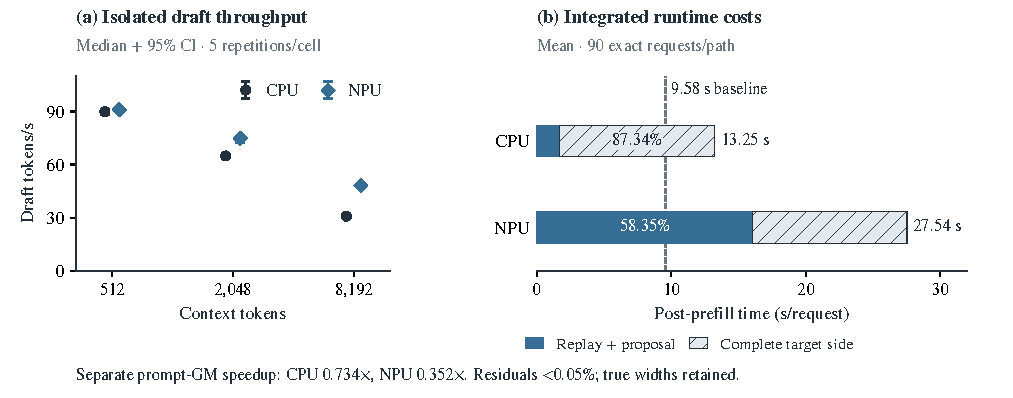
\includegraphics[width=\textwidth]{figures/presentation_v05/pdf/state.pdf}
\caption{\textbf{Isolated draft advantage and complete 358H cost.} A: five-repeat steady-state draft throughput with repetition-bootstrap intervals. B: arithmetic mean post-prefill seconds over 90 exact observations per path, against the shared baseline. NPU's 58.35\% region combines full-prefix replay/reconstruction and proposal; it is inseparable. CPU complete target work is 87.34\%. These bars differ from the prompt-GM speedups in Table~\ref{tab:headlines}; persistence savings are unmeasured.}
\label{fig:state}
\end{figure*}

\subsection{Stateful realization}
\label{sec:state}
On 358H, isolated NPU draft throughput exceeds CPU at tested contexts, but both integrated direct-ID-qualified paths are slower than target-only. Complete committed progress is $C=\HcpuC$ and $\HnpuC$, including correction/bonus. Complete target work consumes \HcpuTarget\% of CPU-path time. The NPU synchronous OpenVINO region combines full-prefix replay/reconstruction and proposal, consuming \HnpuDraft\%; these costs are inseparable. Residual orchestration is \HcpuResidual\% and \HnpuResidual\%.

Figure~\ref{fig:state} describes the measured interface, not NPU capability or a measured persistence benefit. Arithmetic totals give CPU $(\dreal,\rtarget,X)=(\HcpuD,\HcpuR,\HcpuX)$ and NPU $(\HnpuD,\HnpuR,\HnpuX)$, yielding \HcpuAggregate$\times$ and \HnpuAggregate$\times$ in Equation~\ref{eq:normalized}; these are total-time ratios rather than Table~\ref{tab:headlines}'s prompt GMs. With measured progress, target-work and baseline totals fixed, nonnegative draft and residual terms imply $S\le C/\rtarget$: \DerCPUZero$\times$ CPU and \DerNPUZero$\times$ NPU, even if both other terms vanish. Thus draft-only savings cannot reach parity under this accounting. This post-study arithmetic bound is not a prompt-GM bound or an optimization experiment; changing progress or target execution invalidates its fixed assumptions. The later persistent-state/wider-target candidate stops at qualification without formal performance or energy.
